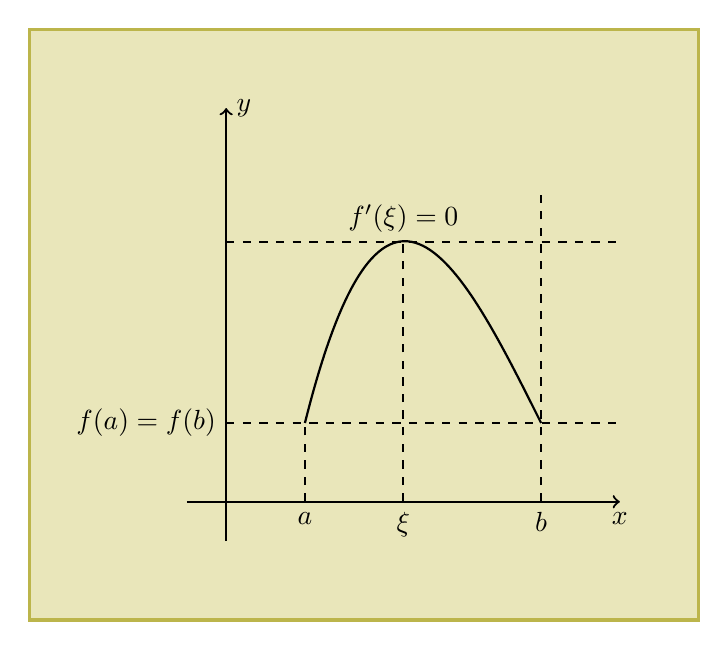
\begin{tikzpicture}
  \draw[draw = olive!60, fill = olive!20, very thick]
    (-2.5, -1.5) rectangle (6, 6);

  \draw[->, thick] (0, -0.5) -- (0, 5)
    node[right] {\(y\)};
  \draw[->, thick] (-0.5, 0) -- (5, 0)
    node[below] {\(x\)};

  \draw[thick] (1, 1) .. controls (2, 5) and (3, 3) .. (4, 1);

  \draw[dashed, thick] (1, 0) -- (1, 1)
    node[pos = 0, below] {\(a\)};
  \draw[dashed, thick] (4, 0) -- (4, 4)
    node[pos = 0, below] {\(b\)};

  \draw[dashed, thick] (0, 1) -- (5, 1)
    node[pos = 0, left] {\(f(a) = f(b)\)};


  \draw[dashed, thick] (0, 3.3) -- (5, 3.3);
  \draw[dashed, thick] (2.25, 0) -- (2.25, 3.3)
    node[pos = 0, below] {\(\xi\)};

  \draw (2.25, 3.3) node[above] {\(f'(\xi) = 0\)};
  \point{2.25, 3.3};

\end{tikzpicture}